%%%%%%%%%%%%%%%%%%%%%%%%%%%%%%%%%%%%%%%%%
% Short Sectioned Assignment
% LaTeX Template
% Version 1.0 (5/5/12)
%
% This template has been downloaded from:
% http://www.LaTeXTemplates.com
%
% Original author:
% Frits Wenneker (http://www.howtotex.com)
%
% License:
% CC BY-NC-SA 3.0 (http://creativecommons.org/licenses/by-nc-sa/3.0/)
%
%%%%%%%%%%%%%%%%%%%%%%%%%%%%%%%%%%%%%%%%%

%----------------------------------------------------------------------------------------
%	PACKAGES AND OTHER DOCUMENT CONFIGURATIONS
%----------------------------------------------------------------------------------------

\documentclass[paper=a4, fontsize=11pt]{scrartcl} % A4 paper and 11pt font size

\usepackage[T1]{fontenc} % Use 8-bit encoding that has 256 glyphs
\usepackage{fourier} % Use the Adobe Utopia font for the document - comment this line to return to the LaTeX default
\usepackage[english]{babel} % English language/hyphenation
\usepackage{amsmath,amsfonts,amsthm} % Math packages

\usepackage{lipsum} % Used for inserting dummy 'Lorem ipsum' text into the template

\usepackage{sectsty} % Allows customizing section commands
\allsectionsfont{\centering \normalfont\scshape} % Make all sections centered, the default font and small caps

\usepackage{fancyhdr} % Custom headers and footers

% use for graph
\usepackage{graphicx} 
\pagestyle{fancyplain} % Makes all pages in the document conform to the custom headers and footers
\fancyhead{} % No page header - if you want one, create it in the same way as the footers below
\fancyfoot[L]{} % Empty left footer
\fancyfoot[C]{} % Empty center footer
\fancyfoot[R]{\thepage} % Page numbering for right footer
\renewcommand{\headrulewidth}{0pt} % Remove header underlines
\renewcommand{\footrulewidth}{0pt} % Remove footer underlines
\setlength{\headheight}{13.6pt} % Customize the height of the header

\numberwithin{equation}{section} % Number equations within sections (i.e. 1.1, 1.2, 2.1, 2.2 instead of 1, 2, 3, 4)
\numberwithin{figure}{section} % Number figures within sections (i.e. 1.1, 1.2, 2.1, 2.2 instead of 1, 2, 3, 4)
\numberwithin{table}{section} % Number tables within sections (i.e. 1.1, 1.2, 2.1, 2.2 instead of 1, 2, 3, 4)

\setlength\parindent{0pt} % Removes all indentation from paragraphs - comment this line for an assignment with lots of text

%----------------------------------------------------------------------------------------
%	TITLE SECTION
%----------------------------------------------------------------------------------------

\newcommand{\horrule}[1]{\rule{\linewidth}{#1}} % Create horizontal rule command with 1 argument of height

\title{	
\normalfont \normalsize 
\textsc{University College cork} \\ [25pt] % Your university, school and/or department name(s)
\horrule{0.5pt} \\[0.4cm] % Thin top horizontal rule
\huge The ethical issues in the use of AI in healthcare \\ % The assignment title
\horrule{2pt} \\[0.5cm] % Thick bottom horizontal rule
}

\author{Kai Deng} % Your name

\date{\normalsize\today} % Today's date or a custom date


\begin{document}
\maketitle % Print the title

%----------------------------------------------------------------------------------------
%	PROBLEM 1
%----------------------------------------------------------------------------------------

\section{Introduction}

\begin{figure}[h]
    \centering
    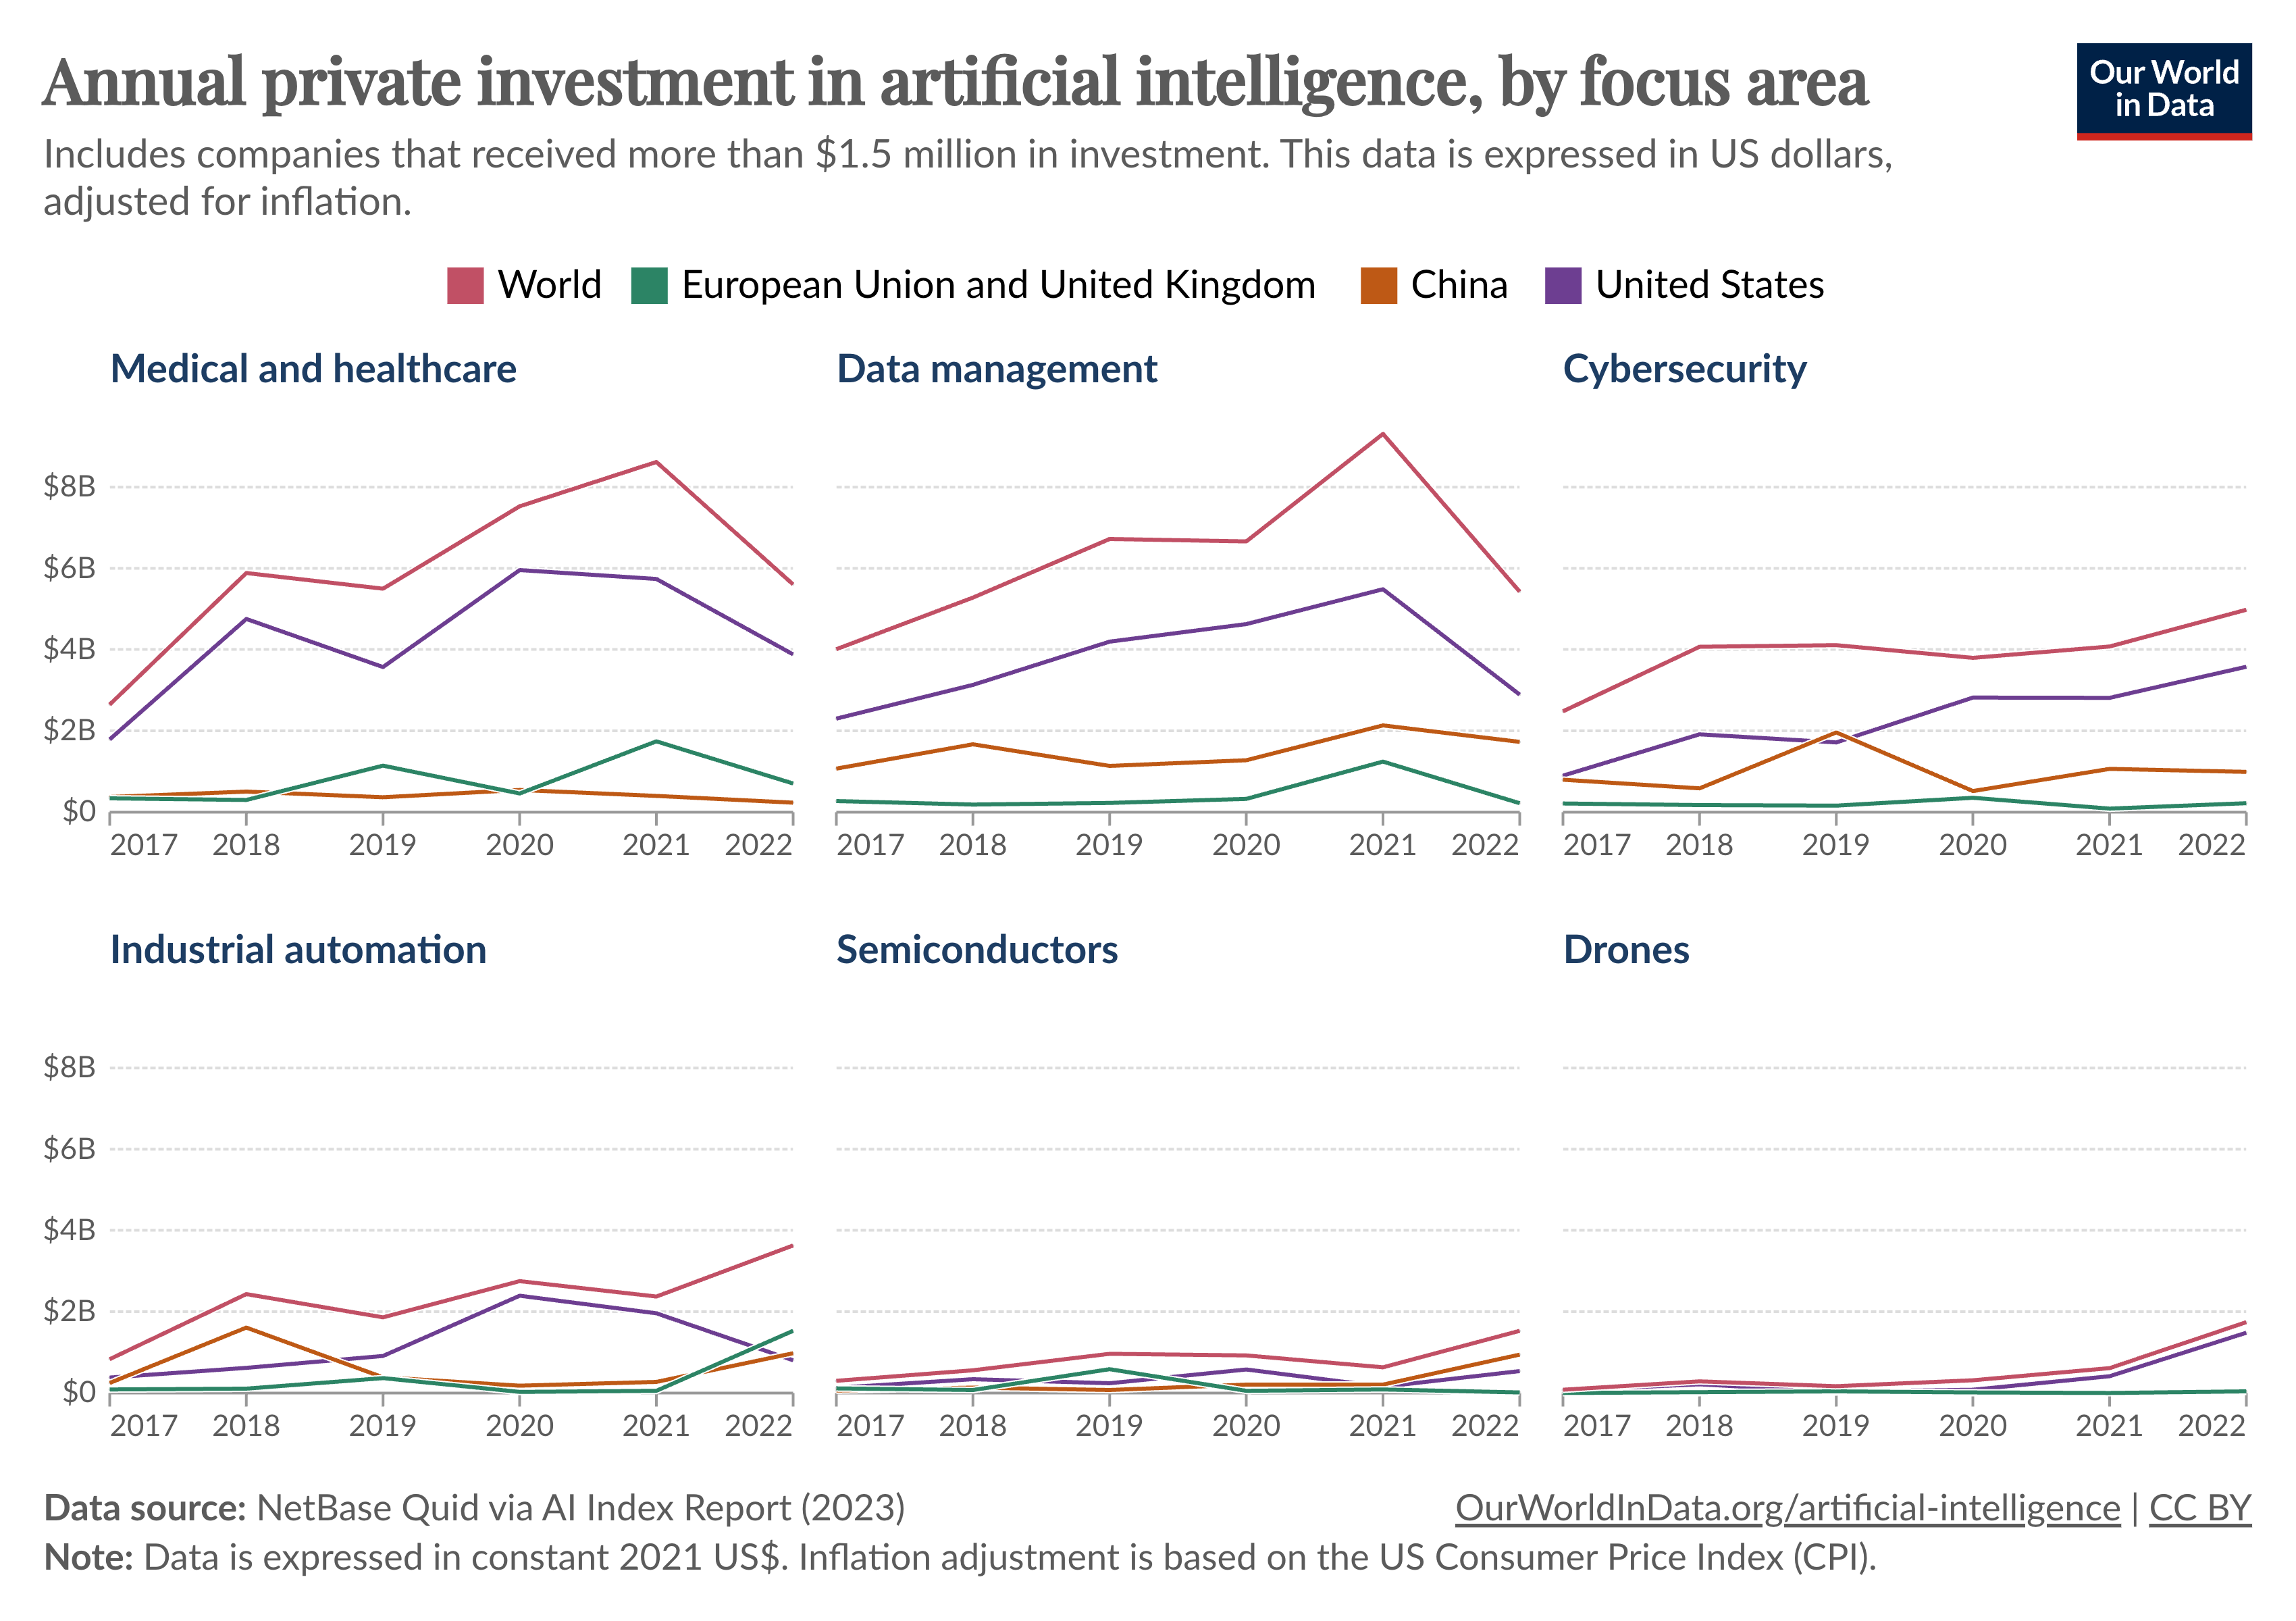
\includegraphics[width=0.5\textwidth]{./data/investegatement.png}
    \caption{This is the title}
    \label{fig:my_picture}
\end{figure}



this is test \cite{chenRethinkingAtrousConvolution2017}


As part of a module for the MA in Digital and Arts and Humanities, i was asked to review a Digital Tool and submit that review to DiRT. I decided to review Overleaf as I have been trying to get away from MS Word for some time and this seemed like a good opportunity to try a different word processor.



Suggested Structure:
Gathering information
In order to begin working with Overleaf, you first need to go to the website and create an account. This was a relatively easy and painless process and I was able to begin working on a document within a couple of minutes.There was a tutorial which suggested itself as soon as you log in but it also gives you the option to just start writing. While I did go through the tutorial it was reassuring to see that they were confident that it was possible to just jump in and start writing. It was also nice that the tutorial was very simple and basic and it took only a couple of minutes though there was an option to go into some things in more detail. The tutorial also directed you to the help menu or to the forum in the even that you needed any help. All in all it was a very nice introduction.


I also had a look for other reviews but there were none that I could find easily. The main reason for this is that Overleaf, is the new brand name for the well known word processing package Write LaTeX.

What I did not know until I eventually found a review is that Overleaf seems to be primarily aimed at Maths students. Had I known this I may have looked elsewhere. All in all I am little confused by this as I was under the impression that LaTeX was not solely aimed at scientists but more generally for those writing any project.


So, Overleaf would seem to be the new kid on the block to some extent albeit with the help of one of the bigger boys. However, there are problems on this front. On the plus side you do not have to download any text editor as is the case with Write LaTeX but that has a downside in that there is no text editor.

I also found difficult once I got past the first few lines. If I tried to mess around with brackets etc I was lost and while the tutorials were helpful, I got the feeling that I would be better off with a fully functional LaTeX editor.

There are other plus points however. Overleaf is free is you are happy with the basement version while you have to pay if you want the bells and whistles. 

There is also a strong community at work who are willing to help and it is not difficult to have queries resolved. This is a positive. 

On the whole though, I was a little disappointed as I expected to get a little more out of it more quickly but I didn't. I looked at one review of Overleaf which was very positive and I think it is worth persevering for a while with it but the jury is out on whether or not I have found the processor that will replace MS Word, for me at least. 




%----------------------------------------------------------------------------------------

\bibliographystyle{plain} % This specifies the style of the bibliography
\bibliography{/Users/dengkai/workspace/papers/latex/config/ref} % This should match the name of your .bib file without the extension



\end{document}

